\documentclass[12pt,letterpaper]{report}
\usepackage{pgf, tikz}
\usetikzlibrary{arrows, automata}

\begin{document}

    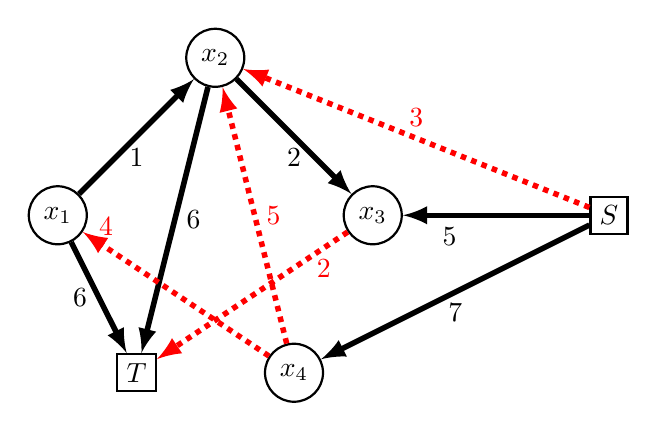
\begin{tikzpicture}[
            > = latex, % arrow head style
            %shorten > = 1pt, % don't touch arrow head to node
            auto,
            node distance = 3cm, % distance between nodes
            line width = 2pt%,
            %thick % line style
        ]

        \tikzstyle{every state}=[
            draw = black,
            thick,
            fill = white,
            minimum size = 4mm
        ]

        \node[state]                              (x1) at (  1 , -2 ) {$x_1$};
        \node[state]                              (x2) at (  3 ,  0 ) {$x_2$};
        \node[state]                              (x3) at (  5 , -2 ) {$x_3$};
        \node[state]                              (x4) at (  4 , -4 ) {$x_4$};
        \node[rectangle,draw,line width = 0.75pt] (S)  at (  8 , -2 ) {$S$};
        \node[rectangle,draw,line width = 0.75pt] (T)  at (  2 , -4 ) {$T$};
        
        %    Head--v        [edge style]         Label[opt]{txt}--v   v--Tail
        \path[->] (S)  edge [red,dotted] node [above]            {3} (x2);
        \path[->] (S)  edge node [below , near end] {5} (x3); % http://tex.stackexchange.com/questions/29712/moving-a-label-along-the-path
        \path[->] (S)  edge node [below]            {7} (x4);
        \path[->] (x1) edge node [below]            {1} (x2);
        \path[->] (x2) edge node [below]            {2} (x3);
        \path[->] (x1) edge node [left]             {6} (T);
        \path[->] (x2) edge node [right]            {6} (T);
        \path[->] (x3) edge [red,dotted] node [below,very near start] {2} (T);
		\path[->] (x4) edge [red,dotted] node [above,very near end]            {4} (x1);
		\path[->] (x4) edge [red,dotted] node [right]            {5} (x2);

        
    \end{tikzpicture}

\end{document}